\documentclass{article}
\usepackage{listings}
\usepackage{color}
\usepackage{amsmath}
\usepackage{mathtools}
\usepackage{amsfonts}
\usepackage{amssymb}
\usepackage{caption}
\usepackage{tabularx}
\usepackage[export]{adjustbox}
\usepackage{polski}
\usepackage{indentfirst}
\usepackage{graphicx}
\usepackage{pdfpages}
\usepackage{float}
\usepackage{gauss}

\DeclareCaptionType{equ}[][List of equations]
\captionsetup[equ]{labelformat=empty}

%script adding bars in matrix
\usepackage{etoolbox}
\makeatletter
\patchcmd\g@matrix
 {\vbox\bgroup}
 {\vbox\bgroup\normalbaselines}% restore the standard baselineskip
 {}{}
\makeatother

\newcommand{\BAR}{%
  \hspace{-\arraycolsep}%
  \strut\vrule % the `\vrule` is as high and deep as a strut
  \hspace{-\arraycolsep}%
}
\definecolor{dkgreen}{rgb}{0,0.6,0}
\definecolor{gray}{rgb}{0.5,0.5,0.5}
\definecolor{mauve}{rgb}{0.58,0,0.82}

\lstset{frame=tb,
  language=Python,
  aboveskip=3mm,
  belowskip=3mm,
  showstringspaces=false,
  columns=flexible,
  basicstyle={\small\ttfamily},
  numbers=none,
  numberstyle=\tiny\color{gray},
  keywordstyle=\color{blue},
  commentstyle=\color{dkgreen},
  stringstyle=\color{mauve},
  breaklines=true,
  breakatwhitespace=true,
  tabsize=3,
  extendedchars=\true,
  inputencoding=utf8x
}

\lstset{literate={ą}{{\k{a}}}1 {ł}{{\l{}}}1 {ń}{{\'n}}1 {ę}{{\k{e}}}1 {ś}{{\'s}}1 {ż}{{\.z}}1 {ó}{{\'o}}1 {ź}{{\'z}}1 {Ą}{{\k{A}}}1 {Ł}{{\L{}}}1 {Ń}{{\'N}}1 {Ę}{{\k{E}}}1 {Ś}{{\'S}}1 {Ż}{{\.Z}}1 {Ó}{{\'O}}1 {Ź}{{\'Z}}1 }

\begin{document}
\title{Sprawozdanie - Metody numeryczne i optymailzacja}
\author{Jakub Andryszczak 259519,\\ Jakub Żak 244255,\\ Maciej Cierpisz 249163}
\date{}
\maketitle

\newpage
\tableofcontents
%Tutaj zaczyna się wstęp

\newpage
\section{Zadanie nr. 1}
Rozwiązać ręcznie i komputerowo metodą eliminacji Gaussa poniższy układ równań
liniowych. Znaleźć elementy podstawowe (pivots).

\begin{equation}
    \begin{cases}
      2u-v=0 \\
     -u+2v-w=0 \\
     -v+2w-z = 0 \\
     -w+2z=5
    \end{cases}\,.
\end{equation}
Rozpocząć proces iteracyjny od zerowej wartości początkowej. Przedtaw krzywe błędów residualnych i aproksymacji rozwiązania (dwa rysunki). Porównaj z rozwiązaniem uzyskanym z eliminacji Gaussa.

Wykorzystano algorytmy metod iteracyjnych:  

Landwebera – jako wartość parametru $\alpha$ przyjęto 0.14 

Jacobiego – macierz A jest przekątniowo dominująca 

Gaussa-Seidela – podobnie jak metoda Jacobiego, ze względu na przekątinowo dominującą macierz 

SOR – jako wartość współczynnika relaksacji przyjęto 0.5 

SD – macierz A jest dodatnio określona 

Kaczmarza – jako współczynnik zbieżności metody, kontrolujący krok iteracji przyjęto 2.9 

Dla każdego z algorytmów wykonano 350 iteracji.  

\begin{figure}[H]
  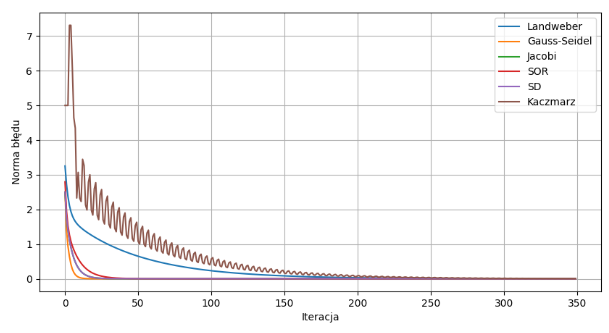
\includegraphics[width=1.5\textwidth, center]{Zad1.1.png}
  \centering
  \captionsetup[Tabela]{name=New Table Name}
  \caption*{Wykres 3.2. Zależność błędu rezydualnego do iteracji}
\end{figure}

\begin{figure}[H]
  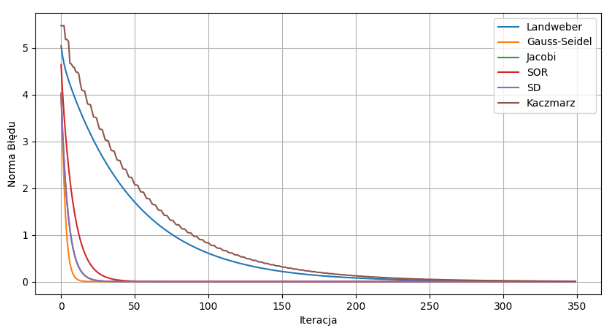
\includegraphics[width=1.5\textwidth, center]{Zad1.2.png}
  \centering
  \captionsetup[Tabela]{name=New Table Name}
  \caption*{Wykres 3.2. Zależność błędu rozwiązania do iteracji}
\end{figure}
\section{Zadanie nr. 2}
Rozwiązać następujący układ równań przy pomocy wybranych metod iteracyjnych:

\begin{equation}
  \begin{cases}
    x_{1}+x_{2}+x_{3}=1 \\
   x_{1}+x_{2}+2x_{3}=2 \\
   x_{1} + 2x_{2} +2x_{3}= 1 
  \end{cases}\,.
\end{equation}
Rozpocznij iteracje od $x^{(0)}=0$. Przedstaw krzywe błędów residualnych i aproksymacji rozwiązania
(dwa rysunki). Porównaj z rozwiązaniem uzyskanym z eliminacji Gaussa. Uzasadnij matematycznie
(na podstawie promienia zbieżności) dlaczego nie udaje się uzyskać zbieżności
niektórymi metodami iteracyjnymi.\newline

W przypadku metody Jacobi wyliczono jego wektor własny
\begin{equation}
  \begin{gmatrix}[b]
    2.1091\\-0.6498\\-1.4593
  \end{gmatrix}
\end{equation}
Wartością spektralną będzie maksymalny moduł wartości własnej, a w naszym wypadku będzie on wynosić p = 2.1091. Oznacza to, iż podczas wykorzystywania tej metody dla podanej macierzy nie jesteśmy w stanie dojść do rozwiązania.\newline

W przypadku metody Gaussa-seidela sprawa wygląda podobnie ponieważ promień zbieżności również jest większy od wartości 1.\newline
\newline
Metoda SOR jest zależna od współczynnika relaksacji $\omega$. Nie udało się znaleźć optymalnej wartości co skutkowało nie znalezieniem żadnego rozwiązania, które spełniałoby warunek zbieżności dla promienia spektralnego.\newline
Metoda Landweber'a zależy od parametru $\alpha$, który kontroluje szybkość zbieżności. W tym wypadku wyznaczamy największą zmodułowaną wartość własną, a następnie podstawiamy do wzoru:
\begin{equation}
  2*|\lambda_{max}(A^TA)|^{-1}=2*17.4887=0.1144
\end{equation}
\newline
Metodę Kaczmarza można wykorzystać dla tego układu równań ponieważ macierz A ma pełny rząd.
\newline
Obie metody dały wyniki przybliżone do rozwiązania uzyskanego za pomocą eliminacji Gaussa.
    \begin{equation}
      x= \begin{gmatrix}[b]
        1\\-1\\1        
      \end{gmatrix}
    \end{equation}
W przypadku metody Landweber'a liczba iteracji wyniosła 746, a dla znalezienia rozwiązania metodą Kaczmarza wystarczyło jedynie 190 iteracji.
    Poniżej przedstawiono wykres zależności błędu residualnego i rozwiązania dla metody Landweber'a i Kaczmarza.
\begin{figure}[h]
  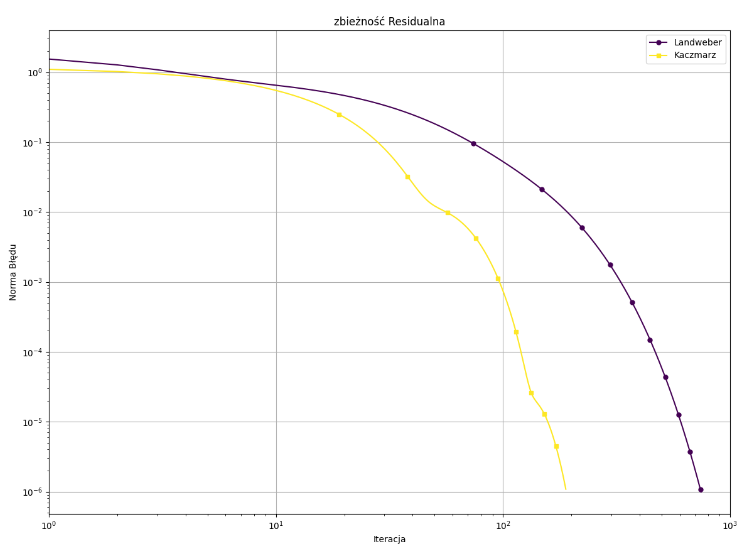
\includegraphics[scale=0.7]{Resco.png}
  \centering
  \captionsetup[Tabela]{name=New Table Name}
  \caption*{Wykres.2.1. Zależność n-tej iteracji metody do błędu residualnego}
\end{figure}
\begin{figure}[h]
  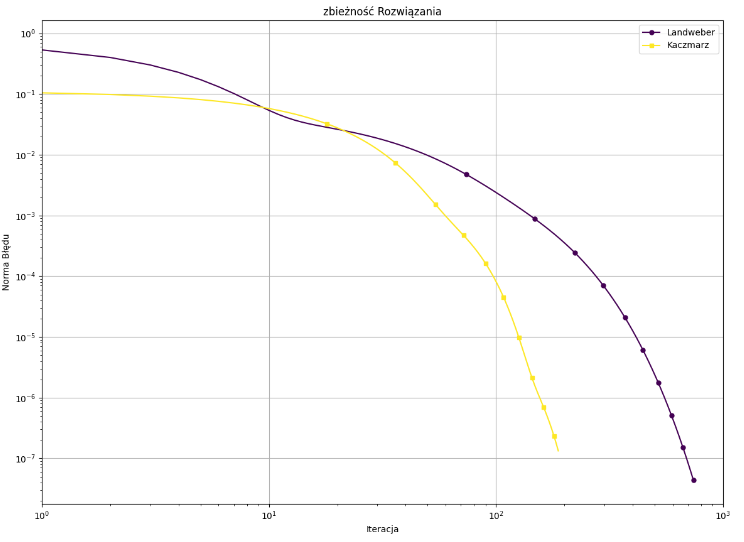
\includegraphics[scale=0.7]{Rozco.png}
  \centering
  \captionsetup[Tabela]{name=New Table Name}
  \caption*{Wykres.2.2. Zależność n-tej iteracji metody do błędu rozwiązania}
\end{figure}

\section{Zadanie nr. 3}
Rozwiąż układ równań liniowych: Ax = b, gdzie: 

 

\begin{equation} 
  A= 
  \begin{gmatrix}[b] 
    1&2&3&4\\ 
    -1&1&2&1\\ 
    0&2&1&3\\ 
    0&0&1&1 
  \end{gmatrix} 
  ,  b= 
  \begin{gmatrix}[b] 
    1&\dots&1 
  \end{gmatrix}^T 
\end{equation} 

 

 

Dla podanego układu równań ustalono, że podane metody iteracyjne nie zadziałają poprawnie: 

Landwebera – brak zbieżności układu 

Jacobiego – brak diagonalnej ani przekątniowej dominacji 

Gaussa-Seidela – analogicznie do metody Jacobiego 

SOR – jako wartość współczynnika relaksacji przyjęto 0.5 

SD – macierz A nie jest dodatnio określona 

Kaczmarza – żadna wartość współczynnika nie pozwala na zbieżność 

Pomimo ustaleń przedstawiono uzyskane przy pomocy algorytmów wykresy na rysunkach: 
\begin{figure}[H]
  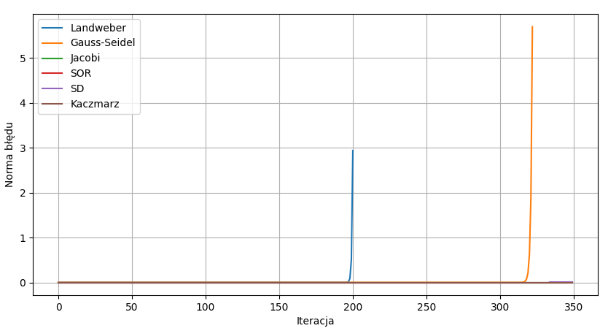
\includegraphics[width=1.5\textwidth, center]{Rysunek.png}
  \centering
  \captionsetup[Tabela]{name=New Table Name}
  \caption*{Wykres 3.1. Zależność błędu rezydualnego do iteracji}
\end{figure}

\begin{figure}[H]
  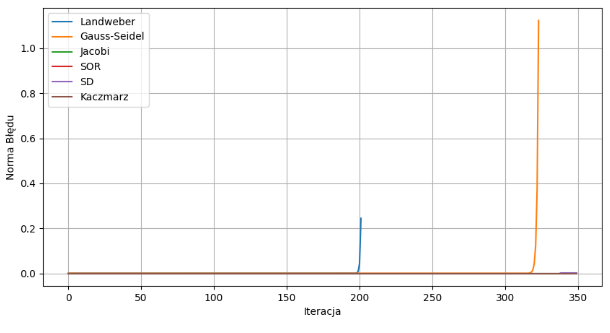
\includegraphics[width=1.5\textwidth, center]{Rys.png}
  \centering
  \captionsetup[Tabela]{name=New Table Name}
  \caption*{Wykres 3.2. Zależność błędu rozwiązania do iteracji}
\end{figure}
\newpage
\section{Zadanie nr. 4}

Niech $A=[a_{ij}] \in R^{NxN}$, gdzie $a_{ij} = \frac{1}{i+j-1}$ (macierz Hilberta) oraz \\
$\begin{gmatrix}[b]
  1&\dots&1
\end{gmatrix}^T\in R^N$.
Rozwiąż układ równań Ax=b dla N= 5,10 i 20, stosując wybrane metody iteracyjne. Rozpocząć interacje od
$x^{(0)}=0$. Przedstaw krzywe błędu residualnego: $r^{(k)}=||b-Ax^{(k)}||_2$.\\

Do zrealizowania zadania zdecydowano się na metody Gaussa-Siedela, Steepest Descent oraz metodę Kaczmarza.
Poniżej matematyczne wyjaśnienie wykorzystanych metod:\\
Metoda Gaussa-Siedela:\\
\begin{equation}
  x^{(k-1)}=S^{-1}(Tx^{(k)}+b)
\end{equation}

\begin{equation}
  A = S-T
\end{equation}

S- macierz dolnotrójkątna,
T- macierz górnotrójkątna

\begin{equation}
  G = s^{-1}T, c=S^{-1}b
\end{equation}
Metoda Steepest Descent:\\
Obliczenie residuum:
\begin{equation}
  r^{(k)}=b-Ax^{(k)}
\end{equation}
Obliczenie kierunku: 
\begin{equation}
  d^{(k)}=-r^{(k)}
\end{equation}
Obliczenie pozycji:
\begin{equation}
  x^{(k+1)}
\end{equation}
Sprawdzenie warunku zatrzymania pętli:\\
Jeśli osiagniemy zadowalający poziom dokładności lub maksymalny poziom iteracji, opuszczamy pętlę.\\
Metoda Kaczmarza:
\begin{equation}
  x_i^{(k+1)}=x_i^{(k)}+\frac{(b_i-\sum_{j=1}^{n}a_{ij}x_j^{(k)})}{a_{ii}},
\end{equation}
gdzie $a_{ij}$ oznacza i-ty wiersz i j-tą kolumne macierzy A, a $b_i$ to i-ta wartość wektora b.\\
Poniżej umieszczono wykresy reprezentujące krzywe błędów residualnych wybranych metod iteracyjnych
dla zadanych wartości N:\\

\begin{figure}[H]%
  \centering%
  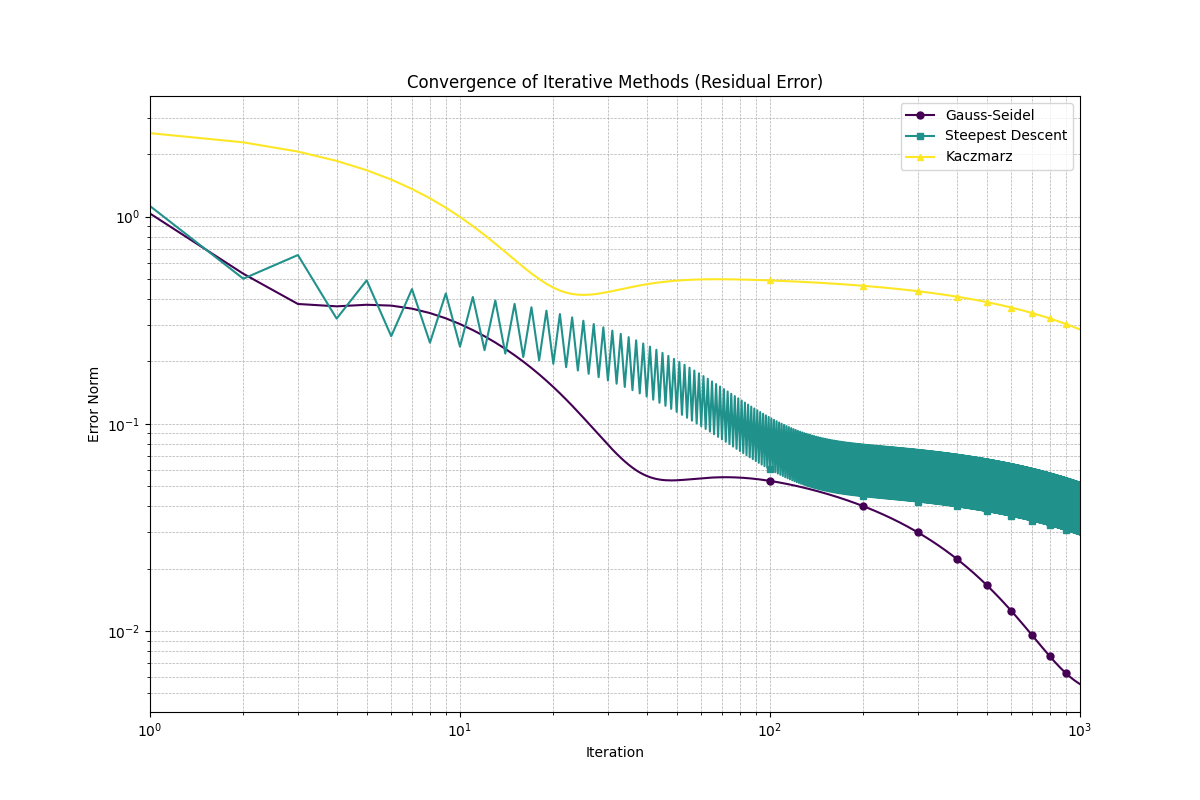
\includegraphics[width=1.5\textwidth, center]{zad4_1.png}%
  \caption*{Wykres.4.1. Krzywe błędów residualnych dla N=5}%
\end{figure}%

\begin{figure}[H]
  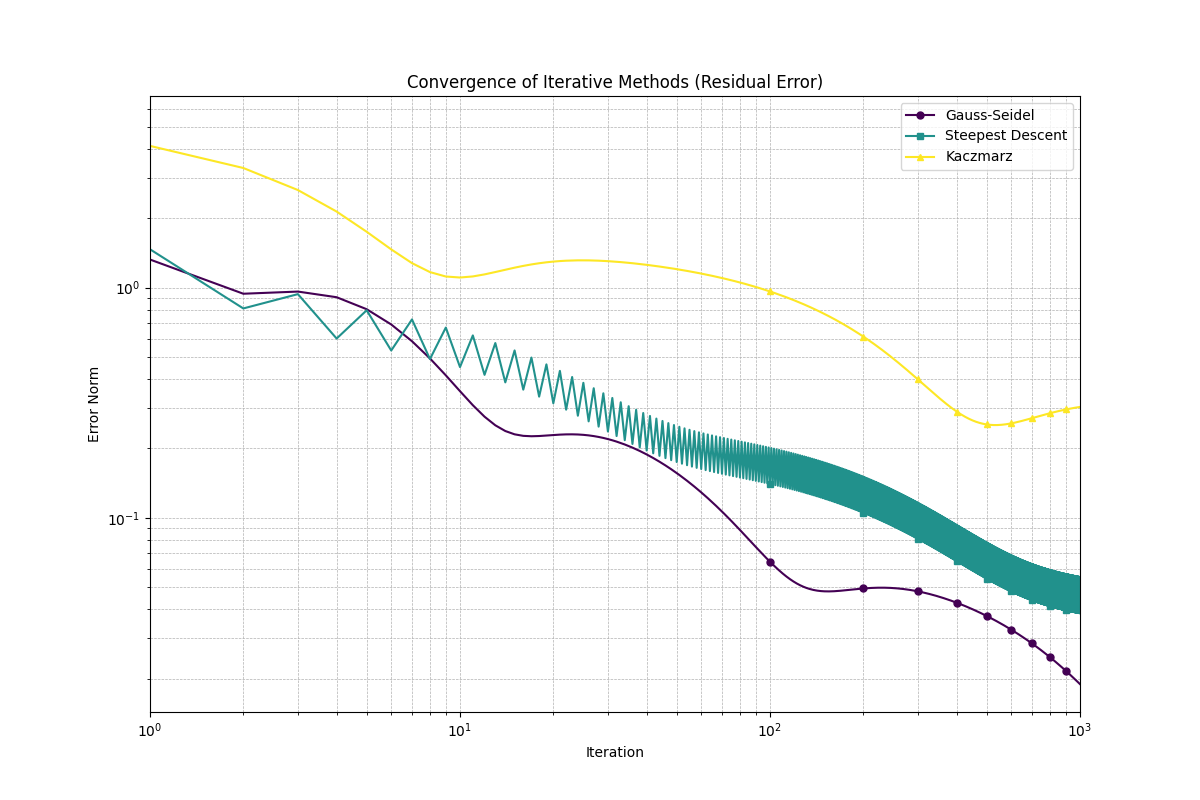
\includegraphics[width=1.5\textwidth, center]{zad4_2.png}
  \centering
  \captionsetup[Tabela]{name=New Table Name}
  \caption*{Wykres.4.2. Krzywe błędów residualnych dla N=10}
\end{figure}

\begin{figure}[H]
  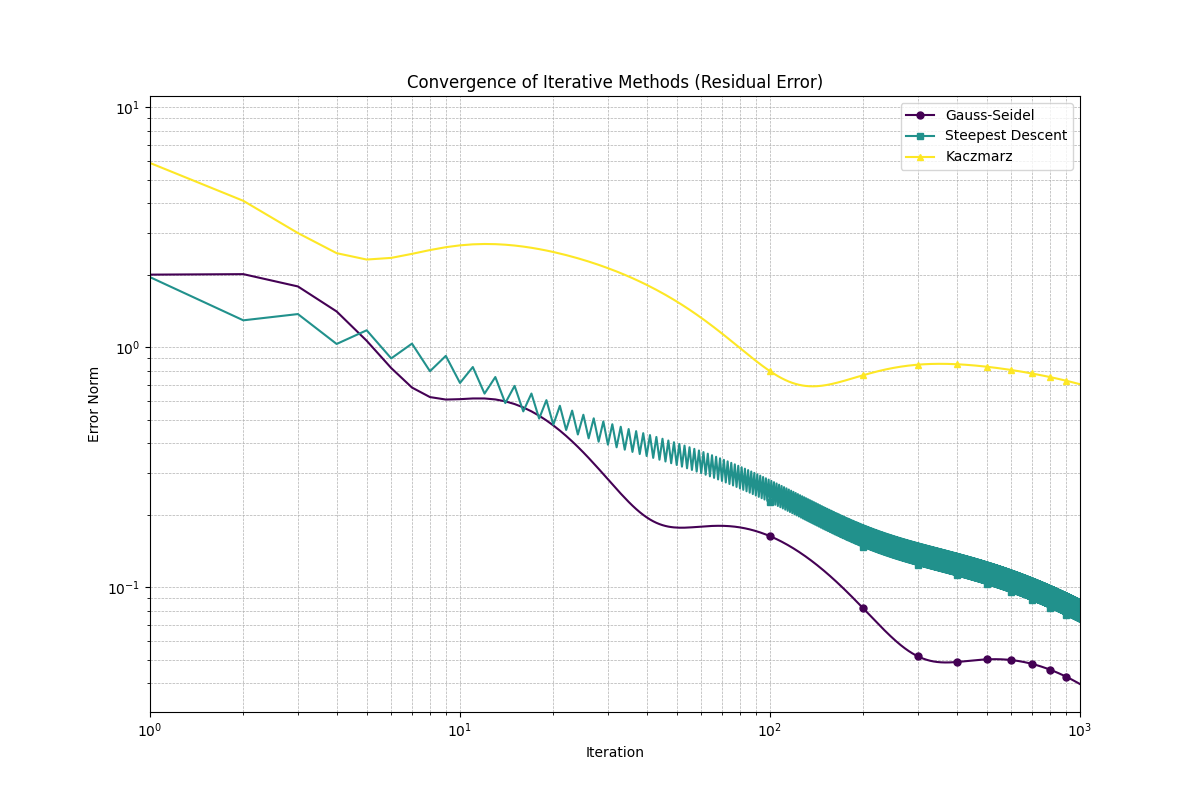
\includegraphics[width=1.5\textwidth, center]{zad4_3.png}
  \centering
  \captionsetup[Tabela]{name=New Table Name}
  \caption*{Wykres.4.3. Krzywe błędów residualnych dla N=20}
\end{figure}

Metoda obarczona najmniejszym błędem rezidualnym dla wszystkich wartości N to metoda Gaussa-Siedela a największym metoda Kaczmarza,
Wyjasnieniem takiego wyniku moze byc fakt iż  macierz Hilberta może zawierać wiersze zerowe.


\section{Zadanie nr. 5}
Niech 
\begin{equation}
  A=
  \begin{gmatrix}[b]
    2&-1&0&\dots\\
    -1&2&\dots&0\\
    0&\dots&2&-1\\
    \dots&0&-1&2
  \end{gmatrix}\in R^{NxN}
  ,
  b=
  \begin{gmatrix}[b]
    1&\dots&1
  \end{gmatrix}^T\in R^N
\end{equation}
Rozwiązać układ równań Ax=b przy pomocy wybranych iteracyjnych solverów dla N = 10,
100, 1000, 10000, 100000. Wykorzystaj reprezentację liczb rzadkich dla dużych macierzy. Dla
każdego N narysować błąd residualny\newline $r^{(k)}=||b-Ax^{(k)}||_2$ w zależności od k-tego kroku iteracyjnego.
Wyjaśnić różnicę w zachowaniu zbieżności.
\newline
Poniżej przedstawiono zależność błędów rozwiązania i rezydualnego w zależności od ilości iteracji.
\begin{figure}[H]
  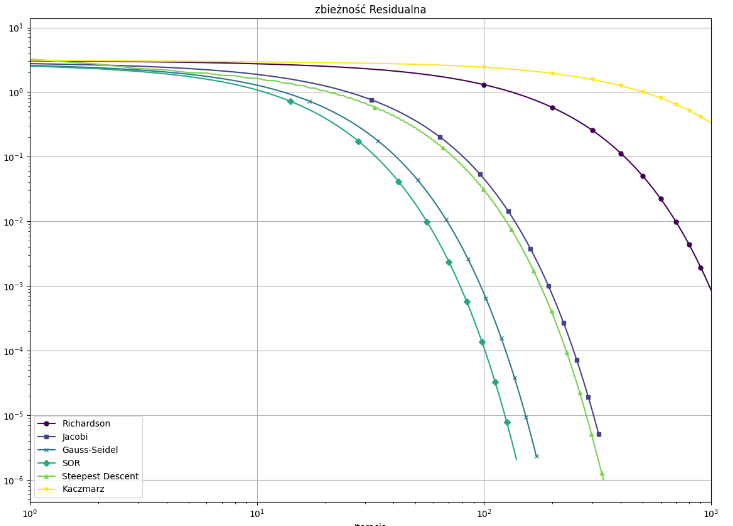
\includegraphics[width=1.5\textwidth, center]{Resco10.png}
  \centering
  \captionsetup[Tabela]{name=New Table Name}
  \caption*{Wykres.5.1. Zależność błędu rezydualnego dla macierzy 10x10 i ilości iteracji= 1000}
\end{figure}
\begin{figure}[H]
  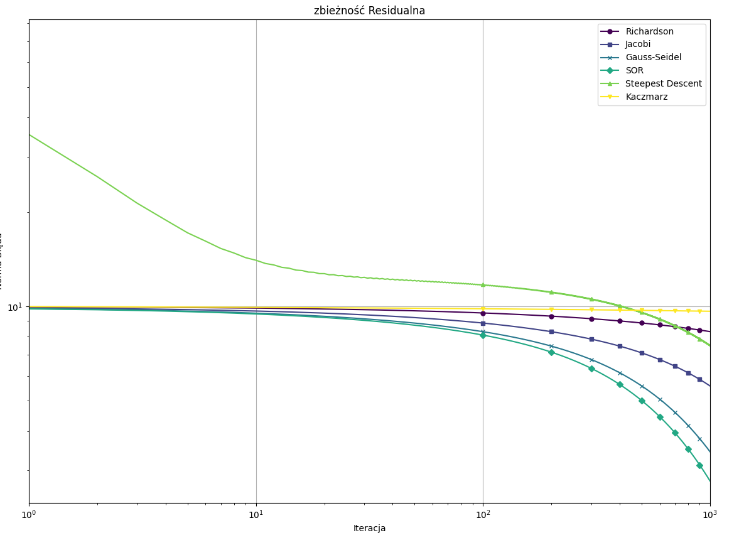
\includegraphics[width=1.5\textwidth, center]{Rezco100.png}
  \centering
  \captionsetup[Tabela]{name=New Table Name}
  \caption*{Wykres.5.2. Zależność błędu rezydualnego dla macierzy 100x100 i ilości iteracji= 1000}
\end{figure}
\begin{figure}[H]
  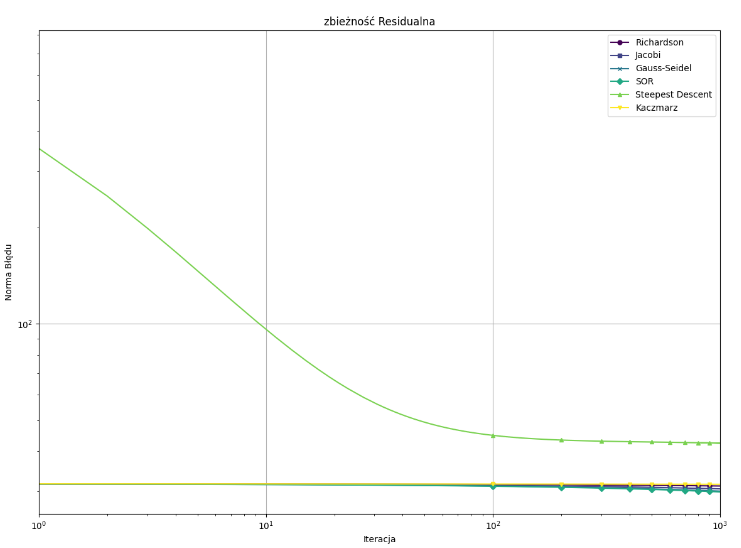
\includegraphics[width=1.5\textwidth, center]{Rezco1000.png}
  \centering
  \captionsetup[Tabela]{name=New Table Name}
  \caption*{Wykres.5.3. Zależność błędu rezydualnego dla macierzy 1000x1000 i ilości iteracji= 1000}
\end{figure}


\begin{figure}[H]
  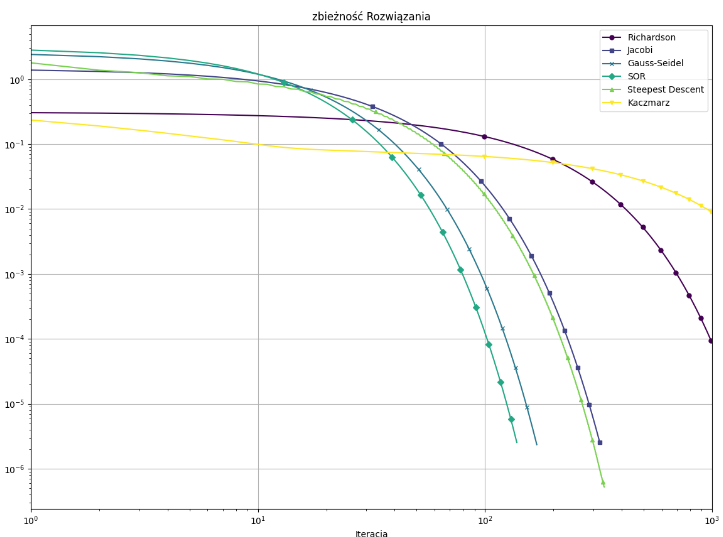
\includegraphics[width=1.5\textwidth, center]{Rozco10.png}
  \centering
  \captionsetup[Tabela]{name=New Table Name}
  \caption*{Wykres.5.1. Zależność błędu rozwiązania dla macierzy 10x10 i ilości iteracji= 1000}
\end{figure}
\begin{figure}[H]
  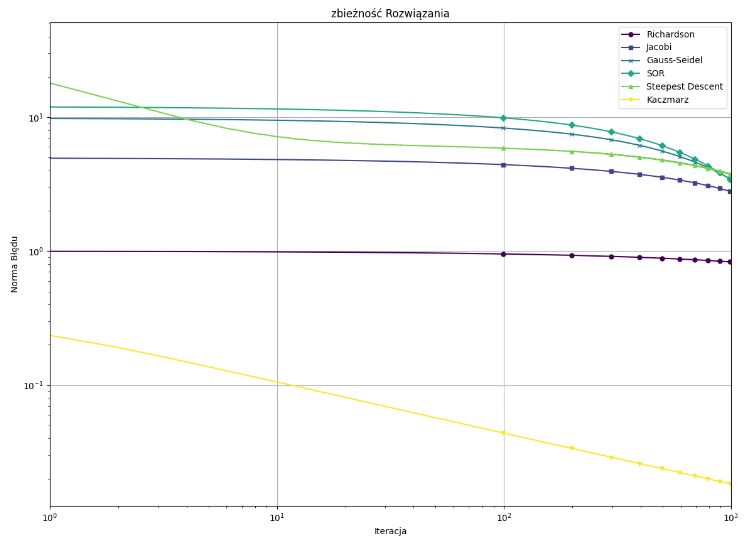
\includegraphics[width=1.5\textwidth, center]{Rozco100.png}
  \centering
  \captionsetup[Tabela]{name=New Table Name}
  \caption*{Wykres.5.1. Zależność błędu rozwiązania dla macierzy 100x100 i ilości iteracji= 1000}
\end{figure}
\begin{figure}[H]
  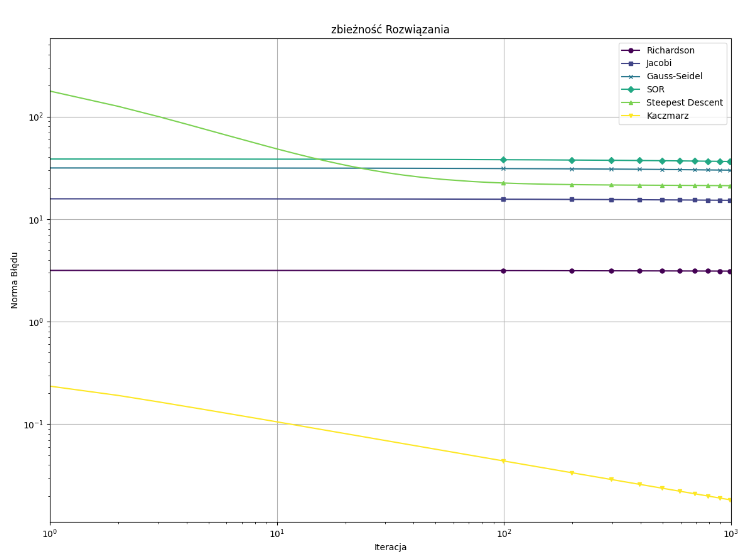
\includegraphics[width=1.5\textwidth, center]{Rozco1000.png}
  \centering
  \captionsetup[Tabela]{name=New Table Name}
  \caption*{Wykres.5.1. Zależność błędu rozwiązania dla macierzy 1000x1000 i ilości iteracji= 1000}
\end{figure}

Niestety ze względu na coraz to dłuższy czas przeliczeń oraz obciążenia komputera jakie za sobą niosły zaprzestano wykonywania zadania tym samym nie wykonując je dla N=10 000 i N= 100 000.
Wraz ze wzrostem wielkości macierzy zwiększała się również liczba iteracji która była potrzebna do wyliczenia prawidłowego rozwiązania o podanej tolerancji. W przypadku macierzy 100x100 tysięczna liczba iteracji nie była w stanie wyliczyć poprawnych wyników.
Ze względu na czas i ograniczenia sprzętowe zwiększono iteracje dla dwóch wybranych metod.
\newline
\begin{center}
  Liczba iteracji dla N=10
\end{center}
Richardson: 361\newline
Jacobi: 323\newline
Gauss-Seidel: 171\newline
SD: 337\newline
Kaczmarz: 6775\newline
\newline
\begin{center}
  Liczba iteracji dla N=100
\end{center}
Richardson: 33107\newline
SD: 33691\newline

\section{Zadanie nr. 6}

Niech $Ax = b$ , $gdzie A = I_N \bigotimes C^TC $, symbol $\bigotimes$ oznacza iloczyn Kroneckera,
$I_N \gets R^{NxN}$ jest macierzą jednostkową, $C \gets R^{MxM}$ jest macierzą losową wygenerowaną z rozkładu normalnego(rand), M=200, N=30, oraz $x~N(0,I_{MN})$ (rozkład normalny - randn).
Porównaj na jednym rysunku krzywe błędu residualnego uzyskane różnymi metodami iteracyjnymi, a na drugim rysunku krzywe błędu aproksymacji rozwiązania $||x^*-x^{(k)}||_2$. Porównaj czas wykonywania się algorytmów.\\

Zdecydowano się na ponowne wykorzystanie algorytmów użytych w zadaniu nr. 4.
Dla kazdego algorytmu wykonano 1000 iteracjii.\\
Poniżej wykaz wykresów przedstawiających krzywe błędów residualnych oraz aproksymacji wybranych algorytmów,
jak i tabela przedstawiająca porównanie czasów wykonywania się algorytmów:

\begin{figure}[H]
  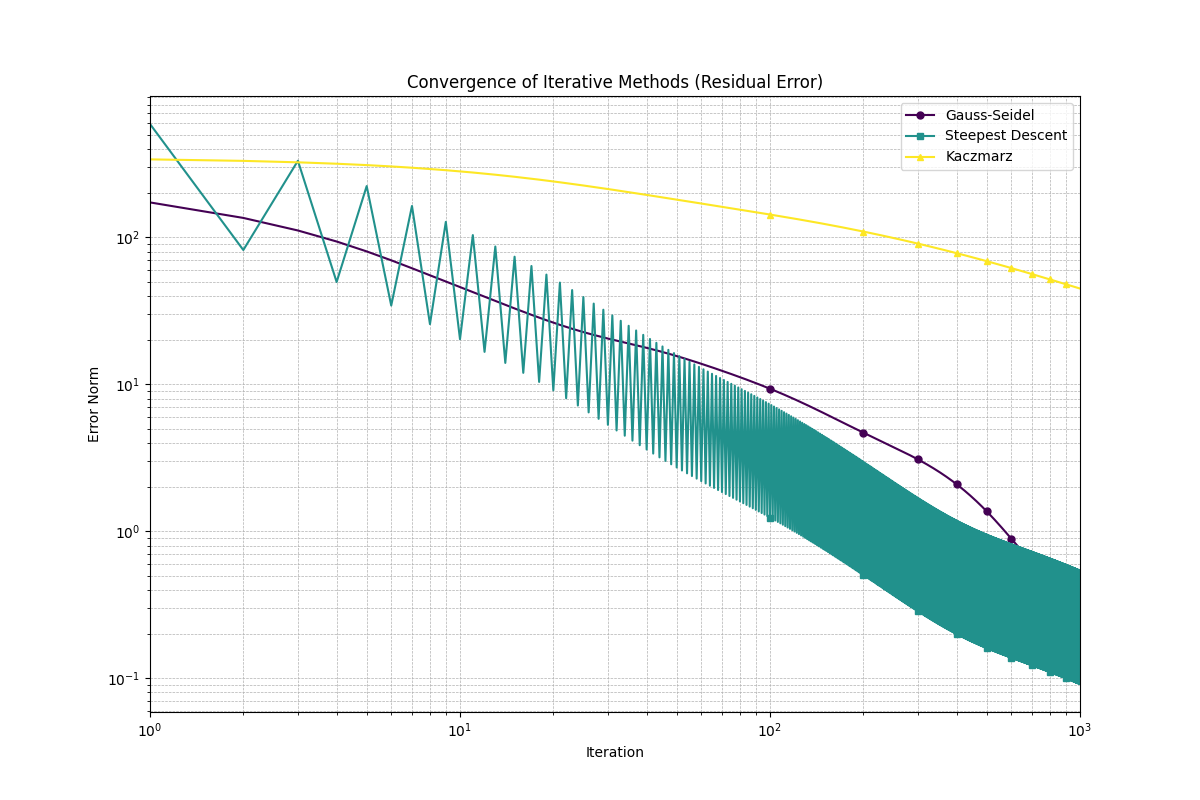
\includegraphics[width=1.5\textwidth, center]{zad6_1.png}
  \centering
  \captionsetup[Tabela]{name=New Table Name}
  \caption*{Wykres.4.2. Krzywe błędów residualnych.}
\end{figure}

\begin{figure}[H]
  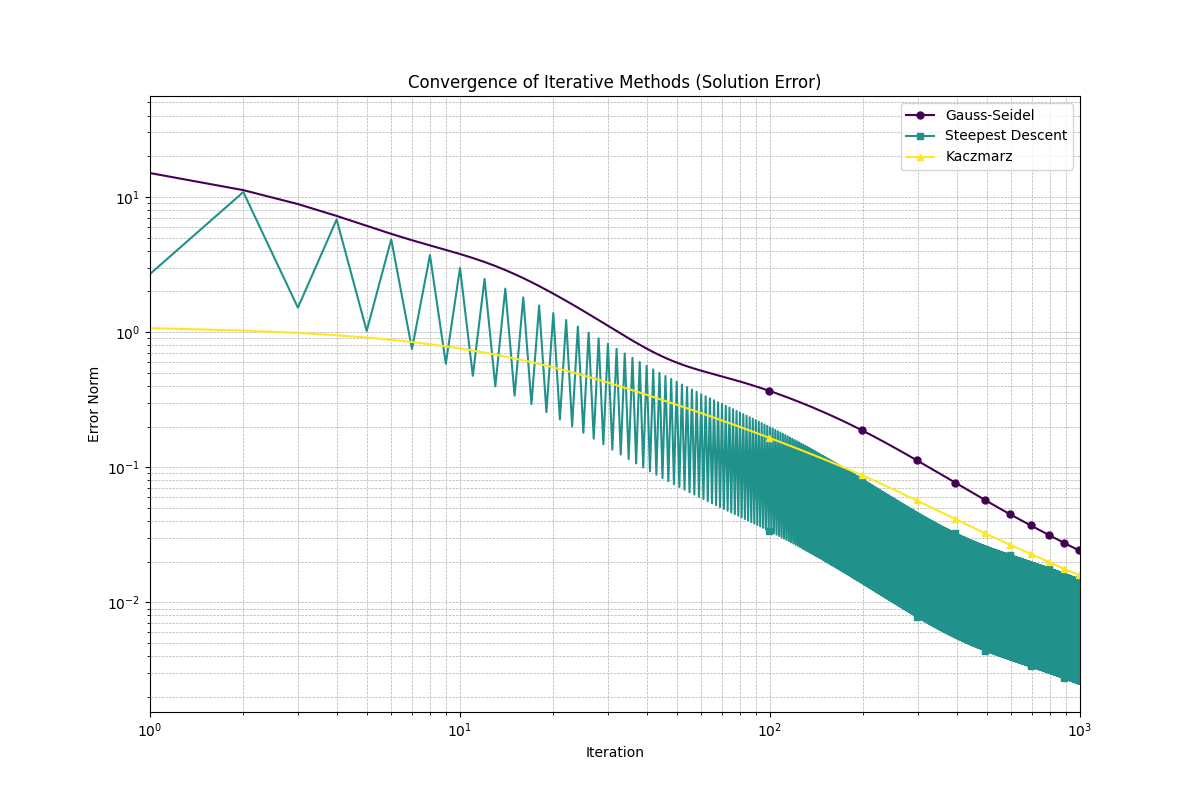
\includegraphics[width=1.5\textwidth, center]{zad6_2.png}
  \centering
  \captionsetup[Tabela]{name=New Table Name}
  \caption*{Wykres.4.2. Krzywe błędów aproksymacji}
\end{figure}

\begin{tabularx}{0.8\textwidth} { 
  | >{\raggedright\arraybackslash}X 
  | >{\centering\arraybackslash}X 
  | >{\raggedleft\arraybackslash}X | }
 \hline
 Metoda & Czas [s]  \\
 \hline
 Gauss-Seidel  & 6522  \\
 \hline
 Steepest Descent  & 12  \\
 \hline
 Kaczmarz  & 94  \\
\hline
\end{tabularx}\\

Długi czas wykonywania metody Gaussa-Seidela moze wynikac z wykorzystania języka wysokiego poziomu oraz ograniczonej wartosci pamieci RAM komputera. Niemniej jednak algorytm ten nie sprawdza sie w przypadku macierzy zainicjowanej iloczynem kroneckera poniewaz wartosci bledu aproksymacji jest największa. Wyniki sugerują, że mimo że metoda Steepest Descent daje najmniejszy błąd aproksymacji, to metoda Kaczmarsza osiąga najlepsze dopasowanie do danych, wyrażone przez najmniejszy błąd residualny. Metoda Gaussa-Siedela wydaje się być najmniej skuteczna z punktu widzenia zarówno błędu aproksymacji, jak i błędu residualnego.

\section{Algorytmy}
\begin{lstlisting}
  def richardson(A, b, x0, tau, max_iter=100, tol=1e-6):
    
    history = []
    x = x0
    for i in range(max_iter):
        r = b - np.dot(A, x)  # obliczenie residuum
        if np.linalg.norm(r) < tol:
            print(f"Iteracja {i}: Znaleziono rozwiązanie z odpowiednią dokładnością.")
            return x, history
        x = x + tau * r  # aktualizacja rozwiązania
        history.append(x.copy())
    print("Nie znaleziono rozwiązania w maksymalnej liczbie iteracji.")
    return x, history
\end{lstlisting}
\begin{lstlisting}
  def landweber(A, b, x0, tau = 0.1, max_iter=100, tol=1e-6):
    history = []
    x = x0
    A_transpose = A.T  # Transpozycja macierzy A

    for i in range(max_iter):
        r = b - np.dot(A, x)  # Obliczenie residuum
        if np.linalg.norm(r) < tol:
            print(f"Iteracja {i}: Znaleziono rozwiązanie z odpowiednią dokładnością.")
            return x, history
        x = x + tau * np.dot(A_transpose, r)  # Aktualizacja rozwiązania z wykorzystaniem gradientu
        history.append(x.copy())
    print("Nie znaleziono rozwiązania w maksymalnej liczbie iteracji.")
    return x,history
\end{lstlisting}
\begin{lstlisting}
  def jacobi(A, b, x0, max_iter=100, tol=1e-6):
    
    history = []
    n = len(b)
    x = x0.copy()
    for it in range(max_iter):
        x_new = np.zeros_like(x)

        for i in range(n):
            s = sum(A[i, j] * x[j] for j in range(n) if i != j)
            x_new[i] = (b[i] - s) / A[i, i]

        if np.linalg.norm(x - x_new, ord=np.inf) < tol:
            print(f"Iteracja {it}: Znaleziono rozwiązanie z odpowiednią dokładnością.")
            return x_new, history
        x = x_new
        history.append(x.copy())

    print("Nie znaleziono rozwiązania w maksymalnej liczbie iteracji.")
    return x, history
\end{lstlisting}
\begin{lstlisting}
  def gauss_seidel(A, b, x0, max_iter=100, tol=1e-6):
    
    history = []
    n = len(b)
    x = x0.copy()
    for it in range(max_iter):
        x_new = np.copy(x)

        for i in range(n):
            s1 = sum(A[i, j] * x_new[j] for j in range(i))
            s2 = sum(A[i, j] * x[j] for j in range(i + 1, n))
            x_new[i] = (b[i] - s1 - s2) / A[i, i]

        if np.linalg.norm(x - x_new, ord=np.inf) < tol:
            print(f"Iteracja {it}: Znaleziono rozwiązanie z odpowiednią dokładnością.")
            return x_new, history
        x = x_new
        history.append(x.copy())

    print("Nie znaleziono rozwiązania w maksymalnej liczbie iteracji.")
    return x, history
\end{lstlisting}
\begin{lstlisting}
  def sor(A, b, x0, omega, max_iter=100, tol=1e-6):
    
    history = []
    n = len(b)
    x = x0.copy()
    for it in range(max_iter):
        x_new = np.copy(x)

        for i in range(n):
            s1 = sum(A[i, j] * x_new[j] for j in range(i))
            s2 = sum(A[i, j] * x[j] for j in range(i + 1, n))
            x_new[i] = (1 - omega) * x[i] + omega * (b[i] - s1 - s2) / A[i, i]

        if np.linalg.norm(x - x_new, ord=np.inf) < tol:
            print(f"Iteracja {it}: Znaleziono rozwiązanie z odpowiednią dokładnością.")
            return x_new, history
        x = x_new
        history.append(x.copy())
    print("Nie znaleziono rozwiązania w maksymalnej liczbie iteracji.")
    return x, history
\end{lstlisting}
\begin{lstlisting}
  def steepest_descent(A, b, x0, max_iter=100, tol=1e-6):
    
    history = []
    x = x0
    r = b - np.dot(A, x)  # początkowe residuum
    for it in range(max_iter):
        Ar = np.dot(A, r)
        alpha = np.dot(r, r) / np.dot(r, Ar)  # obliczenie długości kroku
        x = x + alpha * r  # aktualizacja rozwiązania
        r = b - np.dot(A, x)  # aktualizacja residuum
        if np.linalg.norm(r) < tol:
            print(f"Iteracja {it}: Znaleziono rozwiązanie z odpowiednią dokładnością.")
            return x, history
        history.append(x.copy())
    print("Nie znaleziono rozwiązania w maksymalnej liczbie iteracji.")
    return x, history
\end{lstlisting}
\begin{lstlisting}
  def kaczmarz(A, b, x0, max_iter=100, tol=1e-6):
    
    history = []
    n, m = A.shape
    x = x0.copy()

    for it in range(max_iter):
        for i in range(n):
            ai = A[i, :]
            lambda_i = (b[i] - np.dot(ai, x)) / np.dot(ai, ai)
            x += lambda_i * ai

        r = b - np.dot(A, x)
        if np.linalg.norm(r) < tol:
            print(f"Iteracja {it}: Znaleziono rozwiązanie z odpowiednią dokładnością.")
            return x, history
        history.append(x.copy())

    print("Nie znaleziono rozwiązania w maksymalnej liczbie iteracji.")
    return x, history
\end{lstlisting}
\end{document}